%!TEX root =  main.tex
\setcounter{chapter}{10}
\setcounter{section}{3}
\setcounter{theorem}{0}
\setcounter{equation}{0}

\lectureheader{162}{Calculus II}{The integral test}{\textit{Thomas' Calculus}  \thesection}

\begin{lemma}
If $f$ is a nonnegative, continuous, and decreasing function on the interval $[n, n+1]$, then
\begin{equation*}
0\le f(n) - \int_n^{n+1}f(x)\dee x < f(n) - f(n+1).
\end{equation*}
\end{lemma}

\begin{figure}[h]
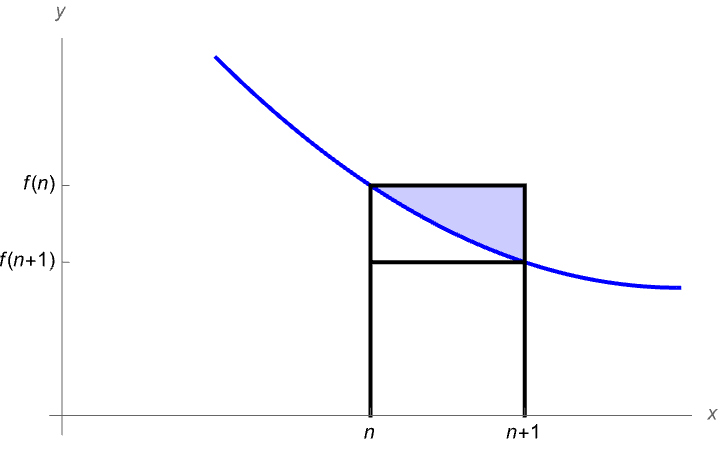
\includegraphics[width=5in]{img/series_integral_diff}
\end{figure}

\newpage

\begin{theorem}[Integral test]
Suppose that $f$ is nonnegative, continuous, and decreasing for all $x\ge k$.
Then
\begin{equation*}
\sum_{n=k}^\infty f(n) \text{ converges }\iff \int_k^\infty f(x)\dee x \text{ converges}.
\end{equation*}
\end{theorem}
\ifdefined\SOLUTION
\SOLUTION[Proof]{
%The idea is ``approximate" the $N$th partial sum
%\begin{equation*}
%S_N = \sum_{n=k}^Nf(n)
%\end{equation*}
%by the integral $\DS\int_k^{N+1}f(x)\dee x$. 
For $N\ge k$, we let
\begin{equation*}
\begin{split}
E_N 
&= S_N - \int_k^{N+1}f(x)\dee x\\
&= \sum_{n=k}^Nf(n) - \int_k^{N+1}f(x)\dee x\\
&= \sum_{n=k}^Nf(n) - \sum_{n=k}^N\int_{n}^{n+1}f(x)\dee x\\
&= \sum_{n=k}^N\left(f(n) - \int_n^{n+1}f(x)\dee x\right).
\end{split}
\end{equation*}
Since the lemma tell us that
\begin{equation*}
0\le f(n) - \int_n^{n+1}f(x)\dee x,
\end{equation*}
it follows that $E_N$ is a monotonic nondecreasing sequence which is bounded below by $0$.
Since the lemma also tells us that
\begin{equation*}
f(n) - \int_n^{n+1}f(x)\dee x < f(n) - f(n+1),
\end{equation*}
it follows that
\begin{equation*}
E_N < \sum_{n=k}^N\Bigg(f(n) - f(n+1)\Bigg) = f(k) - f(N+1) \le f(k),
\end{equation*}
i.e., $E_N$ is bounded above by $f(k)$.
By the monotonic sequence theorem, $E_N\to L$ as $N\to\infty$ for some (finite) nonnegative real number $L<f(k)$.
Therefore, if $\DS\sum_{n=k}^\infty f(n)$ converges, then
\begin{equation*}
\int_k^\infty f(x)\dee x
=\lim_{N\to\infty}\int_k^{N+1}f(x)\dee x
=\lim_{N\to\infty}\left(S_N-E_N\right)
=\sum_{n=k}^\infty f(n) - L.
\end{equation*}
In particular, the improper integral also converges.
Similarly, if $\DS\int_k^\infty f(x)\dee x$ converges, then
\begin{equation*}
\sum_{n=k}^\infty f(n) = \int_k^\infty f(x)\dee x + L.
\end{equation*}
}
\else
\begin{proof}\,

\vspace{6in}
\end{proof}
\fi

\newpage

\begin{definition}
A $p$\textbf{-series} is a series of the form
\begin{equation*}
\sum_{n=1}^\infty \frac{1}{n^p},
\end{equation*}
where $p\in\R$.
The special case when $p=1$ is called the \textbf{harmonic series}.
\end{definition}

\begin{theorem}[$p$-series test]
The $p$-series converges if and only if $p>1$.
In particular, the harmonic series diverges.
\end{theorem}

\ifdefined\SOLUTION
\SOLUTION[Proof]{
Let $p\in\R$.
\begin{equation*}
\lim_{n\to\infty} \frac{1}{n^p} = 
\begin{cases}
\infty &\text{if } p<0,\\
1 & \text{if } p=0.
\end{cases}
\end{equation*}
Therefore, the $p$-series diverges by the test for divergence if $p\le 0$.
Suppose then that $p>0$.
Then $f(x) = 1/x^p$ is nonegative, continuous, and decreasing for all $x\ge 1$.
By the integral test, $\sum_{n=1}^\infty\frac{1}{n^p}$ converges if and only if $\int_1^\infty\frac{\dee x}{x^p}$ converges.
By the $p$-test for integrals $\int_1^\infty\frac{\dee x}{x^p}$ converges if and only if $p>1$.
}
\else
\begin{proof}\,

\vspace{3.25in}
\end{proof}
\fi

\vfill

\begin{remark}[Even simple series are often hard!]\,
\begin{itemize}
\item The proof of the integral test tells us that if $f$ is nonnegative, continuous, and decreasing for all $x\ge k$ and the integral exists, then
\begin{equation*}
%\sum_{n=k}^N f(n) \asymp \int_k^Nf(x)\dee x\quad\text{ as } N\to\infty.
0\le \sum_{n=k}^\infty f(n) - \int_k^\infty f(x)\dee x < f(k).
\end{equation*}
\item It does \underline{not} tell us that the infinite series and the improper integral are equal.  
It tells us that if $f(k)$ is small, then they are good approximations of one another, but most likely they are different.
\item Even though we know how to evaluate the integral $\int_1^\infty\frac{\dee x}{x^p}$ exactly when it exists,
we only know the value of the series $\sum_{n=1}^\infty\frac{1}{n^p}$ for even integers $p\ge 2$.
\item For example, Euler showed
\begin{equation*}
\sum_{n=1}^\infty\frac{1}{n^2} = \frac{\pi^2}{6}.
\end{equation*}
%\item Euler also showed that the divergence of the harmonic series can be used to give a novel proof that there are infinitely many prime numbers.
%\item Riemann would later change the real variable $p$ to a complex variable $s$, and show how the series is connected to a much deeper theory of prime numbers.
\end{itemize}
\end{remark}

\newpage

\begin{example}
Determine whether the following converge or diverge.
\begin{enumerate}
\item $\DS\sum_{n=1}^\infty\frac{1}{n^2+1}$
\ifdefined\SOLUTION
\SOLUTION[Solution]{
Note that $f(x)=1/(x^2+1)$ is positive, continuous, and decreasing for $x\ge 1$.
Therefore, since 
\begin{equation*}
\begin{split}
\int_1^\infty \frac{\dee x}{x^2 + 1} 
&=\lim_{x\to\infty} \int_1^t \frac{\dee x}{x^2 + 1} 
=\lim_{t \to \infty} \arctan{(t)} \Big|_1^t\\
&=\lim_{t\to\infty} \left[ \arctan{t} - \arctan{1}\right] 
=\frac{\pi}{2} - \frac{\pi}{4} = \frac{\pi}{4},
\end{split}
\end{equation*}
it follows that the series $\DS\sum_{n=1}^\infty\frac{1}{n^2+1}$ converges by the integral test.
}
\fi
\vfill
\item $\DS\sum_{n=1}^\infty n\E^{-n^2}$
\ifdefined\SOLUTION
\SOLUTION[Solution]{
Note that $f(x) = x\E^{-x^2}$ is positive, continuous, and decreasing for $x\ge 1$.
Also
\begin{equation*}
\begin{split}
\int_1^\infty x\E^{-x^2}\dee x 
&=\lim_{t\to\infty} \int_1^t x\E^{-x^2} \dee x
=\lim_{t\to\infty} -\frac{1}{2}\int_1^t (-2)x\E^{-x^2} \dee x\\
&=\lim_{t\to\infty} -\frac{1}{2}\E^{-x^2}\Big|_1^t
=\lim_{t\to\infty} \left( \frac{1}{2}\E^{-1} - \frac{1}{2}\E^{-t^2} \right) = \frac{1}{2\E}.
\end{split}
\end{equation*}
Therefore, $\DS\sum_{n = 1}^\infty n\E^{-n^2}$ converges by the integral test.
}
\fi
\vfill
\item $\DS\sum_{n=1}^\infty\frac{1}{2^{\ln n}}$
\ifdefined\SOLUTION
\SOLUTION[Solution]{
Observe that
\begin{equation*}
2^{\ln{(n)}} = \exp \left(\ln{\left(2^{\ln{n}} \right)}\right) = \exp \left( (\ln n)(\ln 2) \right) = \left(\E^{\ln n}\right)^{\ln(2)} = n^{\ln 2}.
\end{equation*}
Therefore,
\begin{equation*}
\sum_{n = 1}^\infty \frac{1}{2^{\ln n}} = \sum_{n = 1}^\infty \frac{1}{n^{\ln 2}}
\end{equation*}
diverges by the $p$-test with $p = \ln (2) < 1$.
}
\fi
\vfill
\end{enumerate}
\end{example}

\newpage

\begin{remark}\,
\begin{itemize}
\item Even when the integral and series both diverge, the proof of the integral test has more to say.
\item Recall from the proof that if $f$ is nonnegative, continuous, and decreasing for all $x\ge k$, then
\begin{equation*}
\left|\sum_{n=k}^N f(n) - \int_k^{N+1} f(x)\dee x\right| < f(k)
\end{equation*}
for all finite $N\ge k$.
\item This means that in the case of divergence, the integral and the sum are asymptotic to one another, i.e., 
\begin{equation*}
S_N = \sum_{n=k}^N f(n) \sim \int_k^{N+1}f(x)\dee x \text{ as } N\to\infty.
\end{equation*}
\item For example, the $N$th harmonic number
\begin{equation*}
H_N = \sum_{n=1}^N\frac{1}{n} \sim \int_1^{N+1}\frac{\dee x}{x} = \ln(N+1) \text{ as }N\to\infty.
\end{equation*}
\end{itemize}
\end{remark}

\vfill

\begin{definition}
The \textbf{Euler--Mascheroni constant} $\gamma$ is defined by 
\begin{equation*}
\gamma = \lim_{N\to \infty}\left(\sum_{n=1}^N\frac{1}{n} - \ln(N+1)\right)\approx 0.57721566.
\end{equation*}
\end{definition}

\vfill

\begin{remark}\,
\begin{itemize}
\item The Euler--Mascheroni constant is one of the most mysterious numbers in mathematics.
\item It shows up all over the place in seemingly disparate areas of mathematics, and to this day we don't even know whether it is rational or irrational.
\item It is also your professor's favorite number.
\item Our proof of the integral test is essentially just a generalization of Euler's proof that $\gamma$ exists.
\end{itemize}
\end{remark}

\newpage

\begin{remark}\,
\begin{itemize}
\item If we know that a series $\DS\sum_{n=0}^\infty a_n$ converges, 
then we can approximate its sum by the $N$th partial sum, i.e., 
\begin{equation*}
\sum_{n=0}^\infty a_n \approx S_N = \sum_{n=0}^N a_n
\end{equation*}
when $N$ is large.
\item The (signed) error in this approximation 
\begin{equation*}
R_N = \sum_{n=0}^\infty a_n - S_N = \sum_{n=N+1}^\infty a_n
\end{equation*}
is called the \textbf{$N$-th remainder} (or \textbf{tail of the series}).
%\item An infinite series converges if and only if one of its tails converges.
%\item This is because 
%\begin{equation*}
%\sum_{n=k}^\infty a_n = \sum_{n=k}^N a_n + \sum_{n=N+1}^\infty a_n = S_N + R_N
%\end{equation*}
%and $S_N$ is just the sum of finitely many real numbers.
%\item So, if we just want to know if the full series converges or diverges, it doesn't matter where we start $n$.
\end{itemize}
\end{remark}

\begin{theorem}[Integral test estimation theorem]
Suppose that $f$ is nonnegative, continuous, and decreasing for all $x\ge N$, and let $a_n=f(n)$.
If $\DS\sum_{n=0}^\infty f(n)$ converges, then 
\begin{equation*}
0\le  \int_{N+1}^\infty f(x)\dee x\le R_N\le \int_{N}^\infty f(x)\dee x.
\end{equation*}
\end{theorem}
\vfill

\begin{remark}
Because the integral test estimation theorem gives a nonnegative lower bound on the $N$th remainder, we can use it to improve our $N$th partial sum approximation.
\end{remark}

\begin{corollary}
Suppose that $f$ is nonnegative, continuous, and decreasing for all $x\ge N$.
If $\DS\sum_{n=0}^\infty f(n)$ converges, then 
\begin{equation*}
\sum_{n=0}^Nf(n) +  \int_{N+1}^\infty f(x)\dee x\le \sum_{n=0}^\infty f(n)\le \sum_{n=0}^Nf(n) +  \int_{N}^\infty f(x)\dee x.
\end{equation*}
\end{corollary}
\vfill

\newpage

\begin{example}
Although we know that $\DS\sum_{n=1}^\infty\frac{1}{n^3}$ exists (i.e., is a finite real number), we don't know very much about it except that Ap\'ery proved that it is an irrational number.
\begin{enumerate}
\item Bound the error in the approximation
\begin{equation*}
\sum_{n=1}^\infty\frac{1}{n^3} \approx \sum_{n=1}^{10}\frac{1}{n^3} = \frac{19164113947}{16003008000} = 1.19753\dots.
\end{equation*}
\ifdefined\SOLUTION
\SOLUTION[Solution]{
We know that $\DS\sum_{n=1}^\infty \frac{1}{n^3}$ converges by the $p$-test with $p=3>1$. 
For every $N\ge 1$,
\begin{equation*}
\int_N^\infty \frac{\dee x}{x^3} 
=\lim_{t\to\infty} \int_N^t \frac{\dee x}{x^3} 
=\lim_{t\to\infty} \frac{-x^{-2}}{-2} \Bigg|_N^t 
=\lim_{t\to\infty}\left( \frac{1}{2N^2} - \frac{1}{2t^2} \right) 
=\frac{1}{2N^2}. 
\end{equation*}
Therefore, the $10$th remainder $R_{10}$ satisfies
\begin{equation*}
0.004\approx \frac{1}{2(11)^2} = \int_{11}^\infty \frac{\dee x}{x^3} \leq R_{10} \leq \int_{10}^\infty \frac{\dee x}{x^3} = \frac{1}{2(10)^2} = 0.005. 
\end{equation*}
}
\else
\fi
\vfill
\item  Now bound the error in the approximation
\begin{equation*}
\begin{split}
\sum_{n=1}^{\infty}\frac{1}{n^3}
&\approx \sum_{n=1}^{10}\frac{1}{n^3} + \int_{11}^\infty\frac{\dee x}{x^3}\\
&= \frac{2326859291587}{1936363968000}\\ 
&= 1.20166\dots.
\end{split}
\end{equation*}
\ifdefined\SOLUTION
\SOLUTION[Solution]{
We know that this is an underestimate with an error that is bounded by
\begin{equation*}
\int_{10}^{11}\frac{\dee x}{x^3} =\frac{1}{2x^2}\Bigg|_{10}^{11} = \frac{1}{2(10)^2} - \frac{1}{2(11)^2}\approx 0.000867769.
\end{equation*}
}
\fi
\vfill
\end{enumerate}
\end{example}

